%%%%%%%%%%%%%%%%%%%%%%%%%%%%%%%%%%%%%%%%%%%%%%%%%%%%%%%%%%%%%%%%%%%%%%
\begin{edXchapter}{Overview}\label{overview}
%%%%%%%%%%%%%%%%%%%%%%%%%%%%%%%%%%%%%%%%%%%%%%%%%%%%%%%%%%%%%%%%%%%%%%

This page may be updated throughout Fall 2016, we recommend to review
this page weekly for changes.

%======================================================================
\begin{edXsection}{About the Course}\label{about-the-course}
%======================================================================


The Big Data Applications and Analytics course is an overview course in
Data Science and covers the applications and technologies (data
analytics and clouds) needed to process the application data. It is
organized around rallying cry: Use Clouds running Data Analytics
Collaboratively processing Big Data to solve problems in X-Informatics.

\end{edXsection}
%======================================================================
\begin{edXsection}{Course Numbers}\label{course-numbers}
%======================================================================


This course is offered for Graduate and Undergraduate students at
Indiana University and as an online course. To Register, for University
credit please go to:

\begin{itemize}
\item  \url{http://registrar.indiana.edu/browser/soc4168/INFO/INFO-I523.shtml}
\item  \url{http://registrar.indiana.edu/browser/soc4168/INFO/INFO-I423.shtml}
\item  \url{http://registrar.indiana.edu/browser/soc4168/ENGR/ENGR-E599.shtml}
\end{itemize}

Please, select the course that is most suitable for your program.

From Student Center:

\begin{quote}
\begin{itemize}
\item
  \begin{description}
  \item[INFO-I 423 - BIG DATA APPLS and ANALYTICS]
  \begin{itemize}
  \itemsep1pt\parskip0pt\parsep0pt
  \item
    34954 online undergraduate students
  \item
    34955 Discussion Friday 9:30 - 10:45AM Informatics East (I2) 150
  \end{itemize}
  \end{description}
\item
  \begin{description}
  \item[INFO-I 523 - BIG DATA APPLS and ANALYTICS]
  \begin{itemize}
  \itemsep1pt\parskip0pt\parsep0pt
  \item
    32863 online graduate students
  \item
    32864 Discussion Friday 9:30 - 10:45AM Informatics East (I2) 150
  \item
    32866 Data Science majors only
  \end{itemize}
  \end{description}
\item
  \begin{description}
  \item[ENGR-E 599 - TOPICS IN INTELLIGENT SYSTEMS ENGINEERING]
  \begin{itemize}
  \itemsep1pt\parskip0pt\parsep0pt
  \item
    36362 online graduate engineering students
  \item
    36363 Discussion Friday 1:00 - 2:15PM Smith Research Center 151E
  \end{itemize}
  \end{description}
\end{itemize}
\end{quote}

From Registrar:

\begin{verbatim}
INFO-I 523  BIG DATA APPLS and ANALYTICS (3 CR)
     CLSD *****          ARR             ARR    ARR       Von Laszewski G          50    0    2
             Above class open to graduates only
             Above class taught online
             Discussion (DIS)
     CLSD 32864          09:30A-10:45A   F      I2 150    Von Laszewski G          50    0    2
             Above class meets with INFO-I 423

INFO-I 523  BIG DATA APPLS and ANALYTICS (3 CR)
    I 523 : P - Data Science majors only
          32866 RSTR     ARR             ARR    ARR       Von Laszewski G          90   72    0
             This is a 100% online class taught by IU Bloomington. No
             on-campus class meetings are required. A distance education
             fee may apply; check your campus bursar website for more
             information
             Above class for students not in residence on the Bloomington
             campus

INFO-I 423  BIG DATA APPLS and ANALYTICS (3 CR)
     CLSD ***** RSTR     ARR             ARR    ARR       Von Laszewski G          10    0    6
             Above class open to undergraduates only
             Above class taught online
             Discussion (DIS)
     CLSD 34955 RSTR     09:30A-10:45A   F      I2 150    Von Laszewski G          10    0    6
             Above class meets with INFO-I 523

ENGR-E 599  TOPICS IN INTELL SYS ENGINEER (3 CR)
       VT: BG DATA APPLICATNS and ANLYTCS ISE
          ***** RSTR     ARR             ARR    ARR       Von Laszewski G          25   25    0
             Above class open to graduate engineering students only
             Above class taught online
             Discussion (DIS)
       VT: BG DATA APPLICATNS and ANLYTCS ISE
          36363 RSTR     01:00P-02:15P   F      HD TBA    Von Laszewski G          25   25    0
             Above class meets Smith Research Center Room 151E
\end{verbatim}

\end{edXsection}
\begin{edXsection}{Meeting Times}\label{meeting-times}

The classes are published online. Residential students at Indiana
University will participate in a discussion taking place at the
following times dependent on which class you are in:

\begin{itemize}
\itemsep1pt\parskip0pt\parsep0pt
\item
  INFO-I 523: Fridays 09:30am - 10:45am EST, I2 150
\item
  ENGR-E 599: Fridays 01:00pm - 02:15pm EST, Research Center Room 151E
\item
  For the 100\% online students a time will be determined
\end{itemize}

\end{edXsection}
\begin{edXsection}{Office Hours}\label{office-hours}

Office hours will be held every week Tue, Thu 10-11am EST.

These are live sessions that will allow you to interact in group or
one-on-one with either an instructor or a TA. Office hours sessions may
be recorded. During these times, we can be reached via zoom with the
following information for the call:

Join from PC, Mac, Linux, iOS or Android:

\begin{itemize}
\itemsep1pt\parskip0pt\parsep0pt
\item
  \url{https://IU.zoom.us/j/195576919}
\end{itemize}

Or Telephone:

\begin{quote}
\begin{itemize}
\itemsep1pt\parskip0pt\parsep0pt
\item
  However as we are most likely sharing documents phone participation
  may not be too useful.
\item
  Dial: +1 646 558 8656 (US Toll) or +1 408 638 0968 (US Toll)
\item
  Meeting ID: 195 576 919
\item
  International numbers available:
  \url{https://IU.zoom.us/zoomconference?m=GUZ8CEVGWPB_312js4gnzkGM_QvcVUy3}
\end{itemize}
\end{quote}

\begin{itemize}
\itemsep1pt\parskip0pt\parsep0pt
\item
  Or a H.323/SIP room system:

  \begin{itemize}
  \itemsep1pt\parskip0pt\parsep0pt
  \item
    H.323: 162.255.37.11 (US West) or 162.255.36.11 (US East)
  \item
    Meeting ID: 195 576 919
  \item
    SIP:
    \href{mailto:195576919@zoomcrc.com}{\nolinkurl{195576919@zoomcrc.com}}
  \end{itemize}
\end{itemize}

Please use a headphone with microphone to increase sound quality.

\end{edXsection}
\begin{edXsection}{Discussions}\label{discussions}

Online discussions will be conducted in piazza at the following URL:

\url{https://piazza.com/iu/fall2016/infoi523/home}

Discussions are conducted in clearly marked folders/topics. For example
``Discussion d1'' will be conducted in the piazza folder ``d1''.
Students are responsible for posting their content to the right folder.
No credit will be given if the post has been filed wrongly.

\end{edXsection}
\begin{edXsection}{Calendar}\label{calendar}

All sessions refer to Sections, Discussions and Units published at the
\href{http://openedx.scholargrid.org/courses/SoIC/INFO-I-523/Fall_2016/courseware/f712efaeae5a4d6ea2c87a0f34e0720b/}{Course
Content Web Page}

\begin{itemize}
\itemsep1pt\parskip0pt\parsep0pt
\item
  This document supersedes any assignment dates and comments regarding
  assignments made in videos or stated elsewhere
\item
  All lectures are assigned Monday's
\item
  All discussions and homework are due Friday's
\end{itemize}

\begin{longtable}[c]{@{}llll@{}}
\toprule
\begin{minipage}[t]{0.16\columnwidth}\raggedright\strut
Date
\strut\end{minipage} &
\begin{minipage}[t]{0.10\columnwidth}\raggedright\strut
Week
\strut\end{minipage} &
\begin{minipage}[t]{0.16\columnwidth}\raggedright\strut
Week
\strut\end{minipage} &
\begin{minipage}[t]{0.45\columnwidth}\raggedright\strut
Descriptions
\strut\end{minipage}\tabularnewline
\begin{minipage}[t]{0.16\columnwidth}\raggedright\strut
08/22/2016
\strut\end{minipage} &
\begin{minipage}[t]{0.10\columnwidth}\raggedright\strut
1
\strut\end{minipage} &
\begin{minipage}[t]{0.16\columnwidth}\raggedright\strut
\begin{quote}
W1
\end{quote}
\strut\end{minipage} &
\begin{minipage}[t]{0.45\columnwidth}\raggedright\strut
S1 Introduction\\S2 Overview\\D1, P1
\strut\end{minipage}\tabularnewline
\begin{minipage}[t]{0.16\columnwidth}\raggedright\strut
08/29/2016
\strut\end{minipage} &
\begin{minipage}[t]{0.10\columnwidth}\raggedright\strut
2
\strut\end{minipage} &
\begin{minipage}[t]{0.16\columnwidth}\raggedright\strut
\begin{quote}
W2
\end{quote}
\strut\end{minipage} &
\begin{minipage}[t]{0.45\columnwidth}\raggedright\strut
S3 Health Info\\D2, D3, P2
\strut\end{minipage}\tabularnewline
\begin{minipage}[t]{0.16\columnwidth}\raggedright\strut
09/05/2016
\strut\end{minipage} &
\begin{minipage}[t]{0.10\columnwidth}\raggedright\strut
3
\strut\end{minipage} &
\begin{minipage}[t]{0.16\columnwidth}\raggedright\strut
Holiday
\strut\end{minipage} &
\begin{minipage}[t]{0.45\columnwidth}\raggedright\strut
Labor Day
\strut\end{minipage}\tabularnewline
\begin{minipage}[t]{0.16\columnwidth}\raggedright\strut
09/05/2016
\strut\end{minipage} &
\begin{minipage}[t]{0.10\columnwidth}\raggedright\strut
3
\strut\end{minipage} &
\begin{minipage}[t]{0.16\columnwidth}\raggedright\strut
\begin{quote}
W3
\end{quote}
\strut\end{minipage} &
\begin{minipage}[t]{0.45\columnwidth}\raggedright\strut
T1 Project and Paper Preparation\\S4 Sport\\D4
\strut\end{minipage}\tabularnewline
\begin{minipage}[t]{0.16\columnwidth}\raggedright\strut
09/12/2016
\strut\end{minipage} &
\begin{minipage}[t]{0.10\columnwidth}\raggedright\strut
4
\strut\end{minipage} &
\begin{minipage}[t]{0.16\columnwidth}\raggedright\strut
\begin{quote}
W4
\end{quote}
\strut\end{minipage} &
\begin{minipage}[t]{0.45\columnwidth}\raggedright\strut
S5 Python, IaaS, FutureSystems\\D5
\strut\end{minipage}\tabularnewline
\begin{minipage}[t]{0.16\columnwidth}\raggedright\strut
09/19/2016
\strut\end{minipage} &
\begin{minipage}[t]{0.10\columnwidth}\raggedright\strut
5
\strut\end{minipage} &
\begin{minipage}[t]{0.16\columnwidth}\raggedright\strut
\begin{quote}
W5
\end{quote}
\strut\end{minipage} &
\begin{minipage}[t]{0.45\columnwidth}\raggedright\strut
S6 Physics\\D6
\strut\end{minipage}\tabularnewline
\begin{minipage}[t]{0.16\columnwidth}\raggedright\strut
09/26/2016
\strut\end{minipage} &
\begin{minipage}[t]{0.10\columnwidth}\raggedright\strut
6
\strut\end{minipage} &
\begin{minipage}[t]{0.16\columnwidth}\raggedright\strut
\begin{quote}
W6
\end{quote}
\strut\end{minipage} &
\begin{minipage}[t]{0.45\columnwidth}\raggedright\strut
S7 Use Cases\\D7
\strut\end{minipage}\tabularnewline
\begin{minipage}[t]{0.16\columnwidth}\raggedright\strut
10/03/2016
\strut\end{minipage} &
\begin{minipage}[t]{0.10\columnwidth}\raggedright\strut
7
\strut\end{minipage} &
\begin{minipage}[t]{0.16\columnwidth}\raggedright\strut
\begin{quote}
W7
\end{quote}
\strut\end{minipage} &
\begin{minipage}[t]{0.45\columnwidth}\raggedright\strut
S8 ??? Viz\\D8
\strut\end{minipage}\tabularnewline
\begin{minipage}[t]{0.16\columnwidth}\raggedright\strut
10/07/2016
\strut\end{minipage} &
\begin{minipage}[t]{0.10\columnwidth}\raggedright\strut
7
\strut\end{minipage} &
\begin{minipage}[t]{0.16\columnwidth}\raggedright\strut
No Lectures
\strut\end{minipage} &
\begin{minipage}[t]{0.45\columnwidth}\raggedright\strut
No Lectures
\strut\end{minipage}\tabularnewline
\begin{minipage}[t]{0.16\columnwidth}\raggedright\strut
10/08/2016
\strut\end{minipage} &
\begin{minipage}[t]{0.10\columnwidth}\raggedright\strut
7
\strut\end{minipage} &
\begin{minipage}[t]{0.16\columnwidth}\raggedright\strut
No Lectures
\strut\end{minipage} &
\begin{minipage}[t]{0.45\columnwidth}\raggedright\strut
No Lectures
\strut\end{minipage}\tabularnewline
\begin{minipage}[t]{0.16\columnwidth}\raggedright\strut
10/09/2016
\strut\end{minipage} &
\begin{minipage}[t]{0.10\columnwidth}\raggedright\strut
7
\strut\end{minipage} &
\begin{minipage}[t]{0.16\columnwidth}\raggedright\strut
No Lectures
\strut\end{minipage} &
\begin{minipage}[t]{0.45\columnwidth}\raggedright\strut
No Lectures
\strut\end{minipage}\tabularnewline
\begin{minipage}[t]{0.16\columnwidth}\raggedright\strut
10/10/2016
\strut\end{minipage} &
\begin{minipage}[t]{0.10\columnwidth}\raggedright\strut
8
\strut\end{minipage} &
\begin{minipage}[t]{0.16\columnwidth}\raggedright\strut
\begin{quote}
W8
\end{quote}
\strut\end{minipage} &
\begin{minipage}[t]{0.45\columnwidth}\raggedright\strut
S9 e-Commerce\\D9
\strut\end{minipage}\tabularnewline
\begin{minipage}[t]{0.16\columnwidth}\raggedright\strut
10/17/2016
\strut\end{minipage} &
\begin{minipage}[t]{0.10\columnwidth}\raggedright\strut
9
\strut\end{minipage} &
\begin{minipage}[t]{0.16\columnwidth}\raggedright\strut
\begin{quote}
W9
\end{quote}
\strut\end{minipage} &
\begin{minipage}[t]{0.45\columnwidth}\raggedright\strut
S10 Clustering\\D10\\PRG1
\strut\end{minipage}\tabularnewline
\begin{minipage}[t]{0.16\columnwidth}\raggedright\strut
10/24/2016
\strut\end{minipage} &
\begin{minipage}[t]{0.10\columnwidth}\raggedright\strut
10
\strut\end{minipage} &
\begin{minipage}[t]{0.16\columnwidth}\raggedright\strut
\begin{quote}
W10
\end{quote}
\strut\end{minipage} &
\begin{minipage}[t]{0.45\columnwidth}\raggedright\strut
S11 Cloud Computing\\D11\\P11
\strut\end{minipage}\tabularnewline
\begin{minipage}[t]{0.16\columnwidth}\raggedright\strut
10/31/2016
\strut\end{minipage} &
\begin{minipage}[t]{0.10\columnwidth}\raggedright\strut
11
\strut\end{minipage} &
\begin{minipage}[t]{0.16\columnwidth}\raggedright\strut
\begin{quote}
W11
\end{quote}
\strut\end{minipage} &
\begin{minipage}[t]{0.45\columnwidth}\raggedright\strut
S13 BigData Technologies\\D12
\strut\end{minipage}\tabularnewline
\begin{minipage}[t]{0.16\columnwidth}\raggedright\strut
11/07/2016
\strut\end{minipage} &
\begin{minipage}[t]{0.10\columnwidth}\raggedright\strut
12
\strut\end{minipage} &
\begin{minipage}[t]{0.16\columnwidth}\raggedright\strut
\begin{quote}
W12
\end{quote}
\strut\end{minipage} &
\begin{minipage}[t]{0.45\columnwidth}\raggedright\strut
S13 BigData Technologies\\D13
\strut\end{minipage}\tabularnewline
\begin{minipage}[t]{0.16\columnwidth}\raggedright\strut
11/14/2016
\strut\end{minipage} &
\begin{minipage}[t]{0.10\columnwidth}\raggedright\strut
13
\strut\end{minipage} &
\begin{minipage}[t]{0.16\columnwidth}\raggedright\strut
\begin{quote}
W13
\end{quote}
\strut\end{minipage} &
\begin{minipage}[t]{0.45\columnwidth}\raggedright\strut
S14 Sensors\\S15 Radar\\TBD Deep Learning\\D14
\strut\end{minipage}\tabularnewline
\begin{minipage}[t]{0.16\columnwidth}\raggedright\strut
11/20/2016
\strut\end{minipage} &
\begin{minipage}[t]{0.10\columnwidth}\raggedright\strut
14
\strut\end{minipage} &
\begin{minipage}[t]{0.16\columnwidth}\raggedright\strut
No Lectures
\strut\end{minipage} &
\begin{minipage}[t]{0.45\columnwidth}\raggedright\strut
Thanksgiving break Starts
\strut\end{minipage}\tabularnewline
\begin{minipage}[t]{0.16\columnwidth}\raggedright\strut
11/27/2016
\strut\end{minipage} &
\begin{minipage}[t]{0.10\columnwidth}\raggedright\strut
14
\strut\end{minipage} &
\begin{minipage}[t]{0.16\columnwidth}\raggedright\strut
No Lectures
\strut\end{minipage} &
\begin{minipage}[t]{0.45\columnwidth}\raggedright\strut
Thanksgiving break Ends
\strut\end{minipage}\tabularnewline
\begin{minipage}[t]{0.16\columnwidth}\raggedright\strut
12/02/2016
\strut\end{minipage} &
\begin{minipage}[t]{0.10\columnwidth}\raggedright\strut
15
\strut\end{minipage} &
\begin{minipage}[t]{0.16\columnwidth}\raggedright\strut
Due Date
\strut\end{minipage} &
\begin{minipage}[t]{0.45\columnwidth}\raggedright\strut
Due Date for papers and projects
\strut\end{minipage}\tabularnewline
\begin{minipage}[t]{0.16\columnwidth}\raggedright\strut
12/12/2016
\strut\end{minipage} &
\begin{minipage}[t]{0.10\columnwidth}\raggedright\strut
16
\strut\end{minipage} &
\begin{minipage}[t]{0.16\columnwidth}\raggedright\strut
Last Class
\strut\end{minipage} &
\begin{minipage}[t]{0.45\columnwidth}\raggedright\strut
Last Homework due
\strut\end{minipage}\tabularnewline
\begin{minipage}[t]{0.16\columnwidth}\raggedright\strut
12/16/2016
\strut\end{minipage} &
\begin{minipage}[t]{0.10\columnwidth}\raggedright\strut
17
\strut\end{minipage} &
\begin{minipage}[t]{0.16\columnwidth}\raggedright\strut
Last Day
\strut\end{minipage} &
\begin{minipage}[t]{0.45\columnwidth}\raggedright\strut
End Date of Semester
\strut\end{minipage}\tabularnewline
\bottomrule
\end{longtable}

\end{edXsection}
\begin{edXsection}{Common Mistakes}\label{common-mistakes}

\begin{itemize}
\itemsep1pt\parskip0pt\parsep0pt
\item
  Starting the Project late.
\item
  Not using gitlab for homework submission
\item
  Not using the 2 column ACM report template
\item
  Not using jabref or endnote for References
\end{itemize}

\end{edXsection}
\begin{edXsection}{Email}\label{email}

We have set up a ticketing system for this class with Google
Collaborative Groups e-mails at

\begin{itemize}
\itemsep1pt\parskip0pt\parsep0pt
\item
  \url{https://groups.google.com/forum/#!forum/big-data-iu-fall-2016-help}
\end{itemize}

This mailinglist is for general help and to contact instructors and TAs.
This mailinglist is shared with all TAs, Dr. von Laszewski, and Dr.
Abdul-Wahid

You can expect a reply from someone on the course staff within 24 hours;
if you do not receive one, please re-send your email.

We also have a general discussion mailing list at

\begin{itemize}
\itemsep1pt\parskip0pt\parsep0pt
\item
  \url{https://groups.google.com/forum/}\#!forum/bigdata-iu-fall-2016
\end{itemize}

If you are writing with questions about the assignments or course
material, please ask on the Discussion Forums so that other students can
benefit from the discussion. For sensitive personal matters, feel free
to email the instructors directly
(\href{mailto:laszewski@gmail.com}{\nolinkurl{laszewski@gmail.com}}).

Class announcements are send to:

\begin{itemize}
\itemsep1pt\parskip0pt\parsep0pt
\item
  \url{https://groups.google.com/forum/}\#!forum/big-data-iu-fall-2016-announce
\end{itemize}

You will be responsible that you verify that you are subscribed to this
list. We will not use canvas e-mail system to communicate with you and
it may only be used initially.

\end{edXsection}
\begin{edXsection}{Systems Usage}\label{systems-usage}

Projects can be executed on Your local computer, a cloud or other
resources you may have access to. This may include:

\begin{itemize}
\itemsep1pt\parskip0pt\parsep0pt
\item
  chameleoncloud.org
\item
  furturesystems.org
\item
  AWS (you will be responsible for charges)
\item
  Azure (you will be responsible for charges)
\item
  virtualbox if you have a powerful computer and like to prototype
\item
  other clouds
\end{itemize}

\end{edXsection}
\begin{edXsection}{Term Paper or Project}\label{term-paper-or-project}

You have a choice to write a term paper or do a software project using
our cloud computing test bed. This will constitute to 40\% of your class
grade.

In case you chose a project your maximum grade could be an A+. However,
an A+ project must be truly outstanding and include an exceptional
project report. Such a project and report will have the potential
quality of being able to be published in a conference.

In case you chose a Term Paper your maximum Grade will be an A-.

\end{edXsection}
\begin{edXsection}{Software Project}\label{software-project}

In case of a software project, we encourage a group project with up to
three members. You can use the
\href{https://piazza.com/class/irqfvh1ctrg2vt}{discussion forum in the
folder project} to form project teams or just communicate privately with
other class members to formulate a team. The following artifacts are
part of the deliverables for a project

\begin{description}
\item[Code:]
You must deliver the code in gitlab. The code must be compilable and a
TA may try to replicate to run your code. You MUST avoid lengthy install
descriptions and everything must be installable from the command line
\item[Project Report:]
A report must be produced while using the format discussed in the Report
Format section. The following length is required:

\begin{itemize}
\itemsep1pt\parskip0pt\parsep0pt
\item
  6 pages, one student in the project
\item
  9 pages, one student in the project
\item
  12 pages, one student in the project
\end{itemize}
\item[Work Breakdown:]
This document is only needed for team projects. A one page PDF document
describing who did what. It includes pointers to the git history that
documents the statistics that demonstrate not only one student has
worked on the project.
\item[License:]
All projects are developed under an open source license such as Apache
2.0 License, or similar. You will be required to add a LICENCE.txt file
and if you use other software identify how it can be reused in your
project. If your project uses different licenses, please add in a
README.rst file which packages are used and which license these packages
have.
\end{description}

\end{edXsection}
\begin{edXsection}{Term Paper}\label{term-paper}

\begin{description}
\item[Project Report:]
A report must be produced while using the format discussed in the Report
Format section. The following length is required:

3-4 pages, one student+ in the project​
\item[Teams:]
Up to three people. You can use the
\href{https://piazza.com/class/irqfvh1ctrg2vt}{discussion forum in the
folder term-project} to build teams.
\item[Term Report:]
A report must be produced while using the format discussed in the Report
Format section. The following length is required:

In case you chose the term paper, you or your team will pick a topic
relevant for the class. You wil write a high quality scholarly paper
about this topic. The following artifacts are part of the deliverables
for a term paper. A report must be produced while using the format
discussed in the Report Format section. The following length is
required:

\begin{itemize}
\itemsep1pt\parskip0pt\parsep0pt
\item
  6 pages, one student in the project
\item
  9 pages, two student in the project
\item
  12 pages, three student in the project
\end{itemize}
\item[Work Breakdown:]
This document is only needed for team projects. A one page PDF document
describing who did what.
\end{description}

\end{edXsection}
\begin{edXsection}{Report Format}\label{report-format}

All reports will be using the ACM proceedings format. The MSWord
template can be found here:

\begin{itemize}
\itemsep1pt\parskip0pt\parsep0pt
\item
  paper-report.docx \textless{}files/paper-report.docx\textgreater{}
\end{itemize}

A LaTeX version can be found at

\begin{itemize}
\itemsep1pt\parskip0pt\parsep0pt
\item
  \url{https://www.acm.org/publications/proceedings-template}
\end{itemize}

however you have to remove the ACM copyright notice in the LaTeX
version.

There will be \textbf{NO EXCEPTION} to this format. In case you are in a
team, you can use either gitlab while collaboratively developing the
LaTeX document or use MicrosoftOne Drive which allows collaborative
editing features. All bibliographical entries must be put into a
bibliography manager such as jabref, endnote, or Mendeley. This will
guarantee that you follow proper citation styles. You can use either ACM
or IEEE reference styles. Your final submission will include the
bibliography file as a separate document.

Documents that do not follow the ACM format and are not accompanied by
references managed with jabref or endnote or are not spell checked will
be returned without review.

Report Checklist:

\begin{itemize}
\itemsep1pt\parskip0pt\parsep0pt
\item
  {[} {]} Have you written the report in word or LaTeX in the specified
  format.
\item
  {[} {]} In case of LaTeX, have you removed the ACM copyright
  information
\item
  {[} {]} Have you included the report in gitlab.
\item
  {[} {]} Have you specified the names and e-mails of all team members
  in your report. E.g. the username in Canvas.
\item
  {[} {]} Have you included all images in native and PDF format in
  gitlab in the images folder.
\item
  {[} {]} Have you added the bibliography file (such as endnote or
  bibtex file e.g. jabref) in a directory bib.
\item
  {[} {]} Have you submitted an additional page that describes who did
  what in the project or report.
\item
  {[} {]} Have you spellchecked the paper.
\item
  {[} {]} Have you made sure you do not plagiarize.
\end{itemize}

\end{edXsection}
\begin{edXsection}{Code Repositories
Deliverables}\label{code-repositories-deliverables}

Code repositories are for code, if you have additional libraries that
are needed you need to develop a script or use a DevOps framework to
install such software. Thus zip files and .class, .o files are not
permissible in the project. Each project must be reproducible with a
simple script. An example is:

\begin{verbatim}
git clone ....
make install
make run
make view
\end{verbatim}

Which would use a simple make file to install, run, and view the
results. Naturally you can use ansible or shell scripts. It is not
permissible to use GUI based DevOps preinstalled frameworks. Everything
must be installable form the command line.

\end{edXsection}
\begin{edXsection}{Prerequisites}\label{prerequisites}

Python or Java experience is expected. The programming load is modest.

In case you elect a programming project we will assume that you are
familiar with the programming languages required as part of the project
you suggest. We will limit the languages to Python and JavaScript if you
like to do interactive visualization. If you do not know the required
technologies, we will expect you to learn it outside of class. For
example, Python has a reputation for being easy to learn, and those with
strong programming background in another general-purpose programming
language (like C/C++, Java, Ruby, etc.) can learn it within a few hours
to days dependent on experience level. Please consult the instructor if
you have concerns about your programming background. In addition, we may
encounter math of various kinds, including linear algebra, probability
theory, and basic calculus. We expect that you know them on an
elementary level. Students with limited math backgrounds may need to do
additional reading outside of class.

In case you are interested in further development of cloudmesh for big
data strong Python or JavaScript experience is needed.

You will also need a sufficiently modern and powerful computer to do the
class work. Naturally if you expect that you want to to the course only
on your cell phone or iPad, or your windows 98 computer, this does not
work. We recommend that you have a relatively new and updated computer
with sufficient memory. In some cases its easier to not use Windows and
for example use Linux via virtualbox, so your machine should have
sufficient memory to comfortably run it. If you do not have such a
machine we are at this time trying to get virtual machines that you can
use on our cloud. However, runtime of these VMs is limited to 6 hours
and they will be terminated after that. Naturally you can run new VMs.
This is done in order to avoid resource ``hogging'' of idle VMs. In
contrast to AWS you are not paying for our VMs so we enforce a rule to
encourage proper community spirit while not occupying resources that
could be used by others. Certainly you can naturally also use AWS or
other clouds where you can run virtual machines, but in that case you
need to pay for the usage yourself.

Please remember that this course does not have a required text books and
the money you safe on this you can be used to buy a new or upgrade your
current computer if needed.

\end{edXsection}
\begin{edXsection}{Learning Outcomes}\label{learning-outcomes}

Students will gain broad understanding of Big Data application areas and
approaches used. This course is a good preparation for any student
likely to be involved with Big Data in their future.

\end{edXsection}
\begin{edXsection}{Grading}\label{grading}

Grading for homework will be done within a week of submission on the due
date. For homework that were submitted beyond the due date, the grading
will be done within 2-3 weeks after the submission. A 10\% grade
reduction will be given. Some homework can not be delivered late (which
will be clearly marked and 0 points will be given if late; these are
mostly related to setting up your account and communicating to us your
account names.)

It is the student's responsibility to upload submissions well ahead of
the deadline to avoid last minute problems with network connectivity,
browser crashes, cloud issues, etc. It is a very good idea to make early
submissions and then upload updates as the deadline approaches; we will
grade the last submission received before the deadline.

Note that paper and project will take a considerable amount of time and
doing proper time management is a must for this class. Avoid starting
your project late. Procastenation does not pay off. Late Projects or
term papers will receive a 10\% grade reduction.

\begin{itemize}
\itemsep1pt\parskip0pt\parsep0pt
\item
  40\% Homework
\item
  40\% Term Paper
\item
  20\% Participation/Discussion
\end{itemize}

Details about the assignments can be found in the Section assignments.

\end{edXsection}
\begin{edXsection}{Academic Integrity Policy}\label{academic-integrity-policy}

We take academic integrity very seriously. You are required to abide by
the Indiana University policy on academic integrity, as described in the
Code of Student Rights, Responsibilities, and Conduct, as well as the
Computer Science Statement on Academic Integrity
(\url{http://www.soic.indiana.edu/doc/graduate/graduate-forms/Academic-Integrity-Guideline-FINAL-2015.pdf}).
It is your responsibility to understand these policies. Briefly
summarized, the work you submit for course assignments, projects,
quizzes, and exams must be your own or that of your group, if group work
is permitted. You may use the ideas of others but you must give proper
credit. You may discuss assignments with other students but you must
acknowledge them in the reference section according to scholarly
citation rules. Please also make sure that you know how to not
plagiarize text from other sources while reviewing citation rules.

We will respond to acts of plagiarism and academic misconduct according
to university policy. Sanctions typically involve a grade of 0 for the
assignment in question and/or a grade of F in the course. In addition,
University policy requires us to report the incident to the Dean of
Students, who may apply additional sanctions, including expulsion from
the university.

Students agree that by taking this course, papers and source code
submitted to us may be subject to textual similarity review, for example
by Turnitin.com. These submissions may be included as source documents
in reference databases for the purpose of detecting plagiarism of such
papers or codes.

\end{edXsection}
\begin{edXsection}{Instructors}\label{instructors}

The course presents lectures in online form given by the instructors
listed bellow. Many others have helped making this material available
and may not be listed here.

For the class the support is provided by

\begin{itemize}
\itemsep1pt\parskip0pt\parsep0pt
\item
  Gregor von Laszewski (PhD)
\item
  Badi Abdhul-Wahid (PhD)
\item
  Jerome Mitchell (Teaching Assistant)
\item
  Prashanth Balasubramani (Teaching Assistant)
\item
  Hyungro Lee (Teaching Assistant)
\end{itemize}

\subsubsection{Gregor von Laszewski}\label{gregor-von-laszewski}

%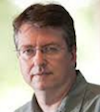
\includegraphics{images/gregor2.png}

Gregor von Laszewski is an Assistant Director of Cloud Computing in the
DSC. He held a position at Argonne National Laboratory from Nov. 1996 --
Aug. 2009 where he was last a scientist and a fellow of the Computation
Institute at University of Chicago. During the last two years of that
appointment he was on sabbatical and held a position as Associate
Professor and the Director of a Lab at Rochester Institute of Technology
focussing on Cyberinfrastructure. He received a Masters Degree in 1990
from the University of Bonn, Germany, and a Ph.D. in 1996 from Syracuse
University in computer science. He was involved in Grid computing since
the term was coined. He was the lead of the Java Commodity Grid Kit
(\url{http://www.cogkit.org}) which provides till today a basis for many
Grid related projects including the Globus toolkit. Current research
interests are in the areas of Cloud computing. He is leading the effort
to develop a simple IaaS client available at as OpenSource project at
\url{http://cloudmesh.github.io/client/}

His Web page is located at \url{http://gregor.cyberaide.org}. To contact
him please send mail to
\href{mailto:laszewski@gmail.com}{\nolinkurl{laszewski@gmail.com}}. For
class related e-mail please use the google group
\url{https://groups.google.com/forum/}\#!forum/big-data-iu-fall-2016-help,
which is shared between all instructors and AIs.

In his free time he teaches Lego Robotics to high school students. In
2015 the team won the 1st prize in programming design in Indiana. If you
like to volunteer helping in this effort please contact him.

He offers also the opportunity to work with him on interesting
independent studies. Current topics include cloudmesh, big data
benchmarking, scientific impact of supercomputer and data centers.

\subsubsection{Dr. Geoffrey Fox}\label{dr.-geoffrey-fox}

%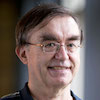
\includegraphics{images/gcf.jpg}

Fox received a Ph.D. in Theoretical Physics from Cambridge University
and is now distinguished professor of Informatics and Computing, and
Physics at Indiana University where he is director of the Digital
Science Center, Chair of Department of Intelligent Systems Engineering
and Director of the Data Science program at the School of Informatics
and Computing. He previously held positions at Caltech, Syracuse
University and Florida State University after being a postdoc at the
Institute of Advanced Study at Princeton, Lawrence Berkeley Laboratory
and Peterhouse College Cambridge. He has supervised the PhD of 68
students and published around 1200 papers in physics and computer
science with an index of 70 and over 26000 citations. He currently works
in applying computer science from infrastructure to analytics in
Biology, Pathology, Sensor Clouds, Earthquake and Ice-sheet Science,
Image processing, Deep Learning, Manufacturing, Network Science and
Particle Physics. The infrastructure work is built around Software
Defined Systems on Clouds and Clusters. The analytics focuses on
scalable parallelism.

He is involved in several projects to enhance the capabilities of
Minority Serving Institutions. He has experience in online education and
its use in MOOCs for areas like Data and Computational Science. He is a
Fellow of APS (Physics) and ACM (Computing).

\subsubsection{Dr. Badi' Abdul-Wahid}\label{dr.-badi-abdul-wahid}

%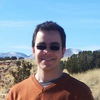
\includegraphics{images/badi.png}

Badi' received a Ph.D. in Computer Science at the University of Notre
Dame under Professor Jesus Izaguirre. The primary focus of his graduate
work was the development of scalable, fault-tolerant, elastic
distributed applications for running Molecular Dynamics simulations.

At Indiana University, Badi' works with the FutureSystems project on a
NIST-funded study whose goal is to understand patterns in the
development and usage of Big Data Analysis pipelines.

\end{edXsection}
\begin{edXsection}{Teaching Assistants}\label{teaching-assistants}

\subsubsection{Hyungro Lee}\label{hyungro-lee}

%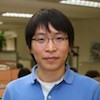
\includegraphics{images/Hyungro.jpg}

Hyungro Lee is a PhD candidate in Computer Science at Indiana University
working with Dr. Geoffrey C. Fox. Prior to beginning the PhD program,
Hyungro worked as a software engineer in the Cyworld Group (social
networking platform in South Korea) at SK Communications, developing
communications platforms including emails, texts and messaging at large
scale to support over 40 million users. From this work he developed an
interest in how distributed systems achieve scalability and high
availability along with managing resources efficiently. He is currently
working on the FutureSystems project to support Big Data Analysis
Software Stacks in Virtual Clusters. He was also working on the
FutureGrid project, an NSF funded significant new experimental computing
grid and cloud test-bed to the research community, together with user
supports. His research interests are parallel and distributed systems,
and cloud computing

\subsubsection{Jerome Mitchell}\label{jerome-mitchell}

%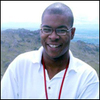
\includegraphics{images/jerome.jpg}

Jerome Mitchell is a Ph.D candidate in computer science at Indiana
University and is interested in coupling the fields of computer and
polar science. He has participated in the United State Antarctic
Program, (USAP), where he collaborated with a multidisciplinary team of
engineers and scientists to design a mobile robot for harsh polar
environments to autonomously collect ice sheet data, decrease the human
footprint of polar expeditions, and enhance measurement precision. His
current work include: using machine learning techniques to help polar
scientists identify bedrock and internal layers in radar imagery. He has
also been involved in facilitating workshops to educate faculty and
students on the importance of parallel and distributed computing at
minority-serving institutions.

\subsubsection{Prashanth Balasubramani}\label{prashanth-balasubramani}

%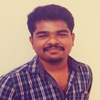
\includegraphics{images/Prashanth.jpg}

Prashanth Balasubramani is an MS student in Computer Science at Indiana
University working with Gregor von Laszewski, Assistant Director of
Cloud Computing at DSC. He has been working under Professor Gregor and
Dr.Geoffrey Fox for the past year as an Associate Instructor for the
course Big Data Analytics and Applications during the Fall 2015 and
Spring 2016 semesters. Before joining Indiana University, he worked as a
ETL developer for Capital One Banking firm (Wipro Technologies,
Bangalore) developing Hadoop MR and Spark jobs for real time migration
of Historical Data into virtual clusters on the Cloud. He is currently
working as an Teaching Assistant for the Big Data Applications and
Analytics course for the Fall 2016 semester. He is also working on NIST
benchmarking project for recording benchmarks on different cloud
platforms His research interests include Big Data applications, Cloud
computing and Data Warehousing.

\end{edXsection}
\begin{edXsection}{Links}\label{links}

This page is published at the following locations:

\begin{itemize}
\itemsep1pt\parskip0pt\parsep0pt
\item
  OpenEdX:
  \url{http://openedx.scholargrid.org/courses/SoIC/INFO-I-523/Fall_2016/about}
\item
  Readthedocs: \url{http://bdaafall2016.readthedocs.io/en/latest/}
\item
  Source: \url{https://gitlab.com/cloudmesh/fall2016}
\end{itemize}
\end{edXsection}

\end{edXchapter}